\documentclass[11pt,a4paper]{article}

\usepackage[T1]{fontenc}
\usepackage{lmodern}
\usepackage[margin=2.3cm]{geometry}
\usepackage{graphicx}
\usepackage{booktabs}
\usepackage{amsmath}
\usepackage{xcolor}
\usepackage{enumitem}
\usepackage[hidelinks]{hyperref}
\usepackage{parskip}

\setlist{itemsep=2pt, topsep=4pt}
\newcommand{\takeaway}[1]{\par\smallskip\noindent\colorbox{black!6}{\parbox{\dimexpr\linewidth-2\fboxsep}{\textbf{In short:} #1}}\par\smallskip}

\title{What Our Results Mean\\[4pt] \large A plain-language guide to the Imvo project's results}
\author{NLP Project 2 group (Lily de Melo, Tawananyasha Kadango, Sally Mohlakola)}
\date{21 October 2026 --- based on the provisional Colab run (pair threshold 0.55, no hand labels yet)}

\begin{document}
\maketitle

\section*{How to read this}
This document explains, step by step, what we measured, why we measured it that way, and what the
numbers tell us. It is written for the group (and anyone else) who wants to understand the results
without reading the code. The paper (\texttt{report/report.pdf}) says the same things in far fewer
words. All numbers come from the files in \texttt{results/}. Everything is \emph{provisional} until the
translated pairs are hand-labelled and the analysis is run once more (Section~\ref{sec:caveats}).

\section{The question}
\emph{Imvo Zabantsundu} (1884--1894) printed a large isiXhosa section and a smaller English section in
every issue. We ask two things:
\begin{enumerate}
  \item \textbf{H1:} Did the two sections carry \emph{different content}, i.e.\ did the isiXhosa readers
  and the English readers get different things to read?
  \item \textbf{H2:} Does the answer change if we first ``modernise'' the 1880s isiXhosa spelling
  (for example \emph{umteto} $\to$ \emph{umthetho})?
\end{enumerate}
H2 matters because modernising spelling looks like harmless cleaning. If it changes the answer, it is a
real analysis choice that people should report, not a cleaning step.

\section{The basic tools}

\paragraph{Chunks.} We cut each page into pieces of 60 words (``chunks''). After removing repeated
adverts and boilerplate, we have 45{,}465 isiXhosa chunks and 22{,}927 English chunks. Issues are split
into train (357 issues), validation (77) and test (77). A whole issue always stays in one split, so the
model is never tested on an issue it has seen.

\paragraph{Embeddings.} A multilingual sentence encoder turns each chunk into a list of 768 numbers (a
vector). Chunks that mean similar things get similar vectors, \emph{even across languages}: a sentence
and its translation should land close together. We use two encoders, LaBSE (main) and multilingual-E5
(a second opinion).

\paragraph{The problem: language gets in the way.} The vectors do not only store meaning, they also
store \emph{which language} the text is in. So if we train a classifier to tell isiXhosa chunks from
English chunks, it will succeed almost perfectly just by spotting the language. That tells us nothing
about content. We saw exactly this: with nothing removed, the classifier tells even
\emph{translations} apart 97\% of the time (Figure~\ref{fig:k}, $k{=}0$). So we must remove the language
signal first, without removing the content differences we want to measure.

\section{Step 1: find translated pairs}
The English section often printed a translation of the isiXhosa editorial. A translated pair is
perfect for us: both sides say the same thing, so \emph{any} difference between their vectors must be
language, not content.

\paragraph{How we find them.} Within each issue, we pair an isiXhosa chunk with an English chunk if
each is the other's most similar chunk (``mutual nearest neighbours''), and keep the pair only if
their similarity is at least 0.55. For LaBSE this keeps 1{,}984 of 8{,}066 candidates (24.6\%):
1{,}373 pairs in training issues, 300 in validation and 311 in test.

\paragraph{Why 0.55 is provisional.} We have not yet hand-checked which pairs are real translations.
Once the team labels a sample, the threshold will be chosen so that at least 90\% of kept pairs are real.
Some current pairs are surely wrong. Section~\ref{sec:synthetic} shows that wrong pairs make our result
\emph{smaller}, not bigger, so this errs on the safe side.

\paragraph{E5 needs its own threshold.} E5's similarities are squeezed into a narrow band (90\% between 0.83 and 0.88),
so 0.55 would keep everything. Instead we keep the same \emph{share} of E5's candidates as LaBSE keeps
(24.6\%), which happens at 0.857.

\section{Step 2: remove the language directions}
For each training pair we subtract the English vector from the isiXhosa vector. Because the content is
the same, each difference is roughly ``the language effect''. We stack all these differences and find
the few directions in which they vary most (a standard tool called SVD). Then we delete those $k$
directions from \emph{every} chunk's vector. Think of it as finding the ``isiXhosa vs English'' axis and
flattening it.

\paragraph{How many directions ($k$)?} We try $k = 0, 1, 2, 4, \dots, 64$. The rule, fixed in advance:
pick the smallest $k$ where, on validation pairs, the classifier can no longer tell translations apart
better than 0.55 (0.50 is a coin flip). If no $k$ gets there, use the largest (64).

\begin{figure}[h]
  \centering
  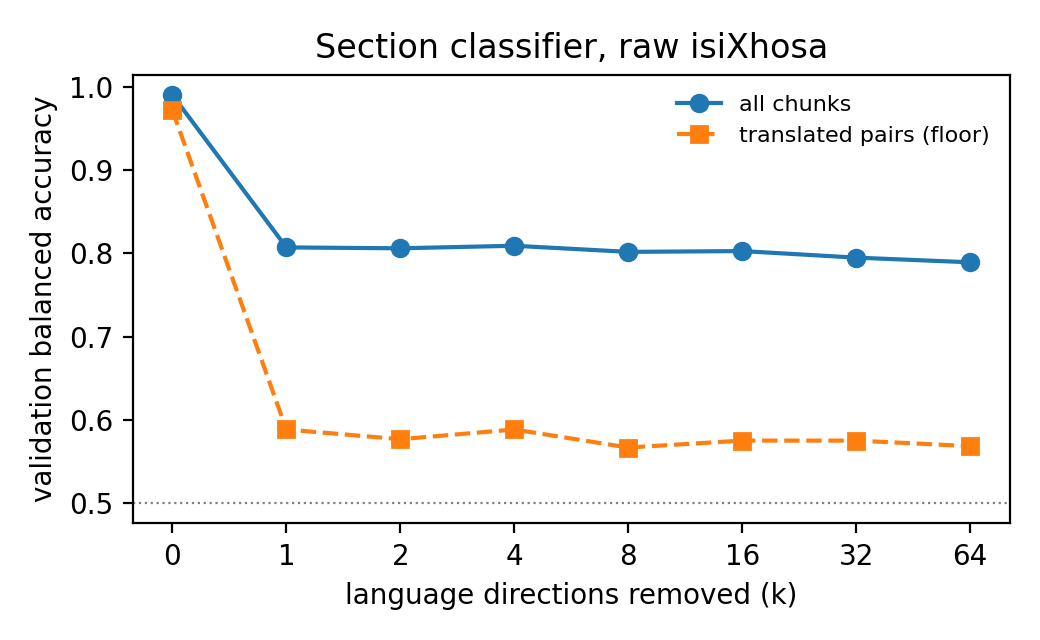
\includegraphics[width=0.62\linewidth]{../results/raw/fig_k_curve.png}
  \caption{Validation accuracy as more language directions are removed (LaBSE, raw text). Orange: how
  well the classifier tells \emph{translations} apart (the floor). Blue: how well it tells \emph{all}
  chunks apart. Removing even one direction kills most of the language signal; the gap between the
  lines stays about 0.2 whatever $k$ we pick.}
  \label{fig:k}
\end{figure}

\paragraph{What happened.} Removing a single direction drops the floor from 0.97 to 0.59. After that it
hardly moves: the lowest it gets is 0.567 (at $k{=}8$), never 0.55. So the fallback rule chose $k{=}64$.
For E5, one direction was enough (validation floor 0.543 at $k{=}1$).

\takeaway{language mostly lives in one direction of the embedding space, but a small amount (about 0.07
above coin-flip for LaBSE) cannot be removed this way. We deal with that leftover in Step 3.}

\section{Step 3: measure content with a classifier}
After removing language, we train a classifier (logistic regression) to predict ``was this chunk in
the isiXhosa section or the English section?'' and test it on the 77 test issues.

\paragraph{Balanced accuracy.} There are twice as many isiXhosa chunks as English ones, so a lazy
classifier could score 66\% by always saying ``isiXhosa''. Balanced accuracy averages the accuracy on
each section separately, so a lazy or random classifier scores 0.50, whatever the class sizes.

\paragraph{The floor and the gap.} We measure balanced accuracy twice:
\begin{itemize}
  \item on \textbf{all} test chunks: this picks up content differences \emph{plus} any leftover language;
  \item on the \textbf{translated pairs} only: here the content is identical, so whatever the classifier
  still gets right must be leftover language. We call this the \textbf{floor}.
\end{itemize}
The \textbf{gap} is the difference:
\[
  \Delta = \text{accuracy on all chunks} - \text{accuracy on translated pairs (floor)}.
\]
This is the key idea of the project. We do not need language removal to be perfect: whatever language
signal is left is measured by the floor and subtracted. Only accuracy \emph{above} the floor counts as
evidence of different content.

\paragraph{Confidence intervals.} To see how much the numbers could wobble, we resample the 77 test
issues with replacement 1{,}000 times (a ``bootstrap'') and recompute. The middle 95\% of those results is
the 95\% confidence interval (CI). If a CI does not include 0, the effect is very unlikely to be noise.

\section{Can we trust the method? The synthetic test}\label{sec:synthetic}
Before trusting a ruler, you measure something whose length you already know. We built fake data with
a built-in content difference of known size $\delta$, plus a fake language signal, and ran three
methods on it:
\begin{itemize}
  \item \textbf{No removal:} reports a gap of 0. The classifier is busy detecting language, so it
  separates even translations perfectly (floor 1.00) and finds no gap above that.
  \item \textbf{Mean-centring} (the common shortcut: subtract each language's average vector): also
  reports 0 at every $\delta$. Subtracting the averages removes the language \emph{and} the average
  content difference, which is exactly what we are trying to measure.
  \item \textbf{Our pair method:} matches an ``oracle'' that sees only content (0.097 vs 0.099 at
  $\delta{=}0.4$). With 40\% wrong pairs mixed in, it still finds the gap but \emph{underestimates} it
  (0.045 vs 0.059).
\end{itemize}

\begin{figure}[h]
  \centering
  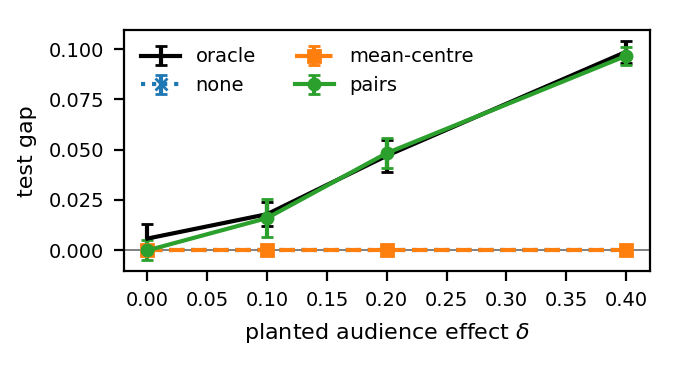
\includegraphics[width=0.55\linewidth]{../report/figures/fig_synthetic.png}
  \caption{Synthetic test: only the pair method (green) recovers the planted gap (black). The other two
  sit on zero.}
  \label{fig:syn}
\end{figure}

\takeaway{the method finds content differences when they exist, the popular alternative cannot, and bad
pairs make our estimate cautious rather than inflated.}

\section{H1 results: the two sections do carry different content}

\begin{table}[h]
\centering
\begin{tabular}{@{}lcccc@{}}
\toprule
Setting & All chunks & Floor & \textbf{Gap} & 95\% CI of gap \\
\midrule
LaBSE, raw text ($k{=}64$) & 0.786 & 0.590 & \textbf{0.196} & 0.167 to 0.224 \\
E5, raw text ($k{=}1$) & 0.877 & 0.618 & \textbf{0.258} & 0.216 to 0.304 \\
LaBSE, stricter pairs (similarity $\geq$ 0.65) & 0.888 & 0.725 & \textbf{0.163} & 0.112 to 0.210 \\
LaBSE, kNN classifier instead & 0.851 & 0.703 & \textbf{0.149} & -- \\
\bottomrule
\end{tabular}
\caption{The content gap on test issues, measured four ways.}
\label{tab:h1}
\end{table}

\paragraph{Reading the table.} With LaBSE, the classifier is right about a chunk's section 78.6\% of the
time (balanced), but on translations, where content is identical, only 59.0\%. The 0.196 difference is
the part explained by content. The CI is far from 0, so this is not noise.

\paragraph{Why we believe it.} The result does not hinge on one choice:
\begin{itemize}
  \item \textbf{Any $k$:} the test gap is between 0.196 and 0.221 for every $k$ from 1 to 64 (also visible in
  Figure~\ref{fig:k}: the two lines stay parallel).
  \item \textbf{Another encoder:} E5 finds an even larger gap (0.258).
  \item \textbf{Stricter pairs:} keeping only pairs with similarity $\geq 0.65$ (fewer, more reliable)
  still gives 0.163.
  \item \textbf{Another classifier:} a $k$-nearest-neighbours classifier, which works very differently
  from logistic regression, gives 0.149.
\end{itemize}

\paragraph{What the different content actually is.} We grouped all chunks into 32 topic clusters
($k$-means on the language-removed vectors) and looked at which clusters are mostly one language. The most
isiXhosa-only clusters are:
\begin{itemize}
  \item \textbf{market price lists} (1{,}211 chunks, \emph{none} in English), e.g.\ \emph{``Inkuku 7d.\ ne 8d.\
  inye; \dots\ Umbona 6/8 ne 7/6 ngekulu''} (chickens 7 or 8 pence each; maize 6s 8d to 7s 6d per hundred, \emph{ngekulu});
  \item \textbf{land-sale and survey notices} (95\% isiXhosa);
  \item \textbf{sport results} (cricket, football) and \textbf{reports of church and society meetings} with
  lists of names.
\end{itemize}
Topics that lean English include liquor licensing, Parliament and government commissions.

We also asked, issue by issue: how different are the topic mixes of the two halves? We compared that
to what we would get if the section labels were shuffled at random. The real halves differ about
twice as much (Jensen--Shannon divergence 0.141 vs 0.067), and 91\% of test issues are above the
shuffled range. E5 shows the same thing even more strongly (0.206 vs 0.041; 100\% of issues).

\paragraph{What this means.} This fits the archive's own description of \emph{Imvo}: the English section was
built around the translated editorial. Our results show what the English readers did \emph{not} get:
the everyday, practical content (prices, notices, sport, community news). The difference is less ``a
different opinion for each audience'' and more ``a fuller newspaper for isiXhosa readers''.

\takeaway{H1 is supported. Even after removing language and subtracting the leftover, the two sections
differ by about 0.2 in balanced accuracy, and the extra isiXhosa content is mostly practical, local
material.}

\section{Modernising the spelling}
Before looking at H2, here is what the modernisation (``normaliser'') does. It uses a word list built
from modern isiXhosa text (Vukuzenzele, Wikipedia, OPUS) and two rules:
\begin{itemize}
  \item \textbf{Aspiration:} 1880s writers often left out the \emph{h} that modern spelling uses
  (\emph{apa} $\to$ \emph{apha}, \emph{pakati} $\to$ \emph{phakathi}, \emph{umteto} $\to$
  \emph{umthetho}). A word is only changed if the old form is (almost) never seen in modern text
  and the new form is common.
  \item \textbf{Prefix joining:} prefixes written as separate words get attached
  (\emph{e Palamente} $\to$ \emph{ePalamente}), but only if the joined form exists in modern text.
\end{itemize}
In total 9.1\% of isiXhosa words are changed: 7.8\% by aspiration (289{,}816 words), 47{,}517 by
joining a prefix to a name and 797 by joining a prefix to an ordinary word. About 96\% of chunks
contain at least one change.

\paragraph{The cost.} The normaliser also rewrites names: \emph{Xosa} $\to$ \emph{Xhosa},
\emph{Tembu} $\to$ \emph{Thembu}, \emph{Mtata} $\to$ \emph{Mthatha}, \emph{Tixo} $\to$ \emph{Thixo}
(God). In all, 191 words that the writers almost always capitalised (19{,}917 occurrences) are changed;
most are names, a few are institutions such as \emph{Rulumente} (government). These are correct modern spellings, but
they overwrite how the writers spelled their own people, places and God. The archive deliberately did
not spell-check the text, because the spelling of the period differs from today's.

\section{H2 results: modernisation nudges the gap, but not the conclusion}

\paragraph{How we decide.} We do not just ask ``is the change different from zero?'', because a
non-significant result does not prove there is no change. Instead we set a margin in advance: a change
smaller than $\pm 0.02$ in the gap counts as ``no practical difference''. We then look at the 90\% CI of
the change (the standard choice for this kind of equivalence test):
\begin{itemize}
  \item whole CI inside $-0.02$ to $+0.02$ $\Rightarrow$ \textbf{equivalent} (modernising is safe);
  \item CI excludes 0 $\Rightarrow$ \textbf{different} (modernising changes the answer);
  \item otherwise $\Rightarrow$ \textbf{inconclusive}.
\end{itemize}
To see which rule does what, we also ran each rule on its own (an ``ablation''). All variants reuse the
raw text's pairs and $k$, so the only thing that changes is the spelling.

\begin{table}[h]
\centering
\begin{tabular}{@{}lccccc@{}}
\toprule
Variant & All & Floor & Gap & Change in gap (90\% CI) & Verdict \\
\midrule
raw & 0.786 & 0.590 & 0.196 & -- & -- \\
modern (both rules) & 0.784 & 0.571 & 0.214 & $+0.018$ ($-0.003$ to $+0.037$) & inconclusive \\
aspiration only & 0.783 & 0.569 & 0.213 & $+0.017$ ($-0.001$ to $+0.038$) & inconclusive \\
prefix joins only & 0.786 & 0.600 & 0.187 & $-0.009$ ($-0.024$ to $+0.006$) & inconclusive \\
\midrule
E5: raw & 0.877 & 0.618 & 0.258 & -- & -- \\
E5: modern & 0.864 & 0.593 & 0.271 & $+0.013$ ($-0.015$ to $+0.039$) & inconclusive \\
\bottomrule
\end{tabular}
\caption{Effect of modernisation on the gap (test issues).}
\label{tab:h2}
\end{table}

\paragraph{Reading the table.} Every verdict is ``inconclusive'': the CIs include 0, but they also
stretch past $+0.02$. So we cannot say modernisation is harmless, and we cannot say it definitely
changes things. But the pattern is clear and consistent:
\begin{itemize}
  \item Full modernisation \emph{raises} the gap by about 0.018, and almost all of that comes from the
  aspiration rule (0.017). Prefix joining does little.
  \item E5 moves the same way (+0.013), so it is not a quirk of one encoder.
\end{itemize}

\paragraph{Why does the gap go up? The most useful finding.} Look at the ``All'' column: it barely moves
(0.786 $\to$ 0.784; the change is $-0.002$, 95\% CI $-0.007$ to $+0.004$). So modernising does
\emph{not} change how well the classifier can tell the sections apart. What changes is the
\emph{floor}: it drops from 0.590 to 0.571. In other words, after modernisation, translations look
more alike, so less leftover language leaks into the floor, and the gap (all minus floor) grows.

A second measurement agrees: the average similarity between translated pairs goes \emph{up} after
modernisation (by 0.005, CI 0.003 to 0.007). That is a cautious result, because the pairs were
chosen using the raw text, which gives raw an advantage, and modern still wins.

This makes sense linguistically: restoring the missing \emph{h} turns many 1880s words into the
modern words the encoder learned from, so the encoder ``understands'' more of the isiXhosa and lines it
up better with the English.

\paragraph{What this means.} Modernising the spelling does not change \emph{what} the newspaper says;
it changes how well our \emph{measuring tool} can read it. The headline answer to H1 stays the same
(about 0.2 either way), but the exact number moves by about as much as our ``no difference'' margin.
So spelling modernisation is a choice that should be reported, and ideally run both ways, rather than
treated as invisible cleaning.

\takeaway{H2 is formally inconclusive. Modernising raises the measured gap slightly (by about 0.02,
mostly via aspiration) by making the two languages line up better, not by changing the content. The
conclusion of H1 survives either way.}

\section{What to be careful about}\label{sec:caveats}
\begin{enumerate}
  \item \textbf{Everything is provisional.} The 0.55 pair threshold was a guess. After the team labels
  pairs, the threshold is re-chosen and the analysis is run once more. The numbers will shift a little.
  \item \textbf{The floor never reached 0.55 for LaBSE.} Some language is left (test floor 0.590, CI 0.561
  to 0.621). This is why we subtract the floor instead of assuming it is 0.5.
  \item \textbf{Stricter pairs raised the floor} (0.590 $\to$ 0.725). With only 362 training pairs, the
  64 language directions are estimated less reliably. The gap still held (0.163), but this check is
  weaker than it looks.
  \item \textbf{The pairs are not a typical sample.} 72\% of paired isiXhosa chunks come from page 2
  (where the editorial is), against 49\% of all isiXhosa chunks; 43\% come from 1885--86. The floor is
  measured on editorial-style text.
  \item \textbf{Part of the gap may be layout, not topic.} Price lists and tables look very different from
  prose. Our boilerplate filter did not remove them. So H1 is best stated as ``the sections printed
  different \emph{kinds of material}'', not ``the editor had different opinions for each audience''.
  \item \textbf{The topic clusters are fuzzy} (silhouette score 0.008, where 1 would be perfectly separated).
  They are good for describing the difference, not for exact counts.
  \item \textbf{Two E5 oddities.} Its classifier chose the weakest regularisation we allowed
  ($C{=}1000$, the edge of the search range), and its kNN classifier found only a small gap (0.046) after removing language. E5's
  content signal seems to lie along a straight-line direction that logistic regression finds but
  ``nearest neighbours'' does not. LaBSE has neither issue.
  \item \textbf{One metric we ignore on purpose.} The comparison figure also shows ``P@1'' (how often a
  chunk's translation is its nearest match). Raw scores exactly 1.0 by construction, because the pairs
  were chosen in the raw space. Its drop for modern spelling is an artefact, so we do not report it.
\end{enumerate}

\section{The whole story in one paragraph}
Once we remove the language signal using translated pairs, and subtract whatever language is left
over, a classifier can still tell \emph{Imvo}'s isiXhosa and English sections apart well above chance
(gap 0.196 with LaBSE, 0.258 with E5). The difference holds across every setting we tried, and it is
mostly practical content (prices, land notices, sport, meetings) that only isiXhosa readers got. The
common shortcut, mean-centring, would have reported no difference at all. Modernising the 1880s
spelling leaves that conclusion intact, but it nudges the measured gap up by about 0.02, almost
entirely through the aspiration rule. It does this by helping the encoder line up the two languages,
not by changing the content. Since modernisation also rewrites the names of people, places and God,
we recommend reporting results on both raw and modernised text.

\end{document}
